\section{Signaling Server}
Although \index{WebRTC}{WebRTC} is a \index{peer-to-peer}{peer-to-peer} communication technology it requires some sort of signaling server to connect peers. 

The following figure shows a complete communication for a video conference.
\begin{figure}[H]
	\hspace*{-3cm}
	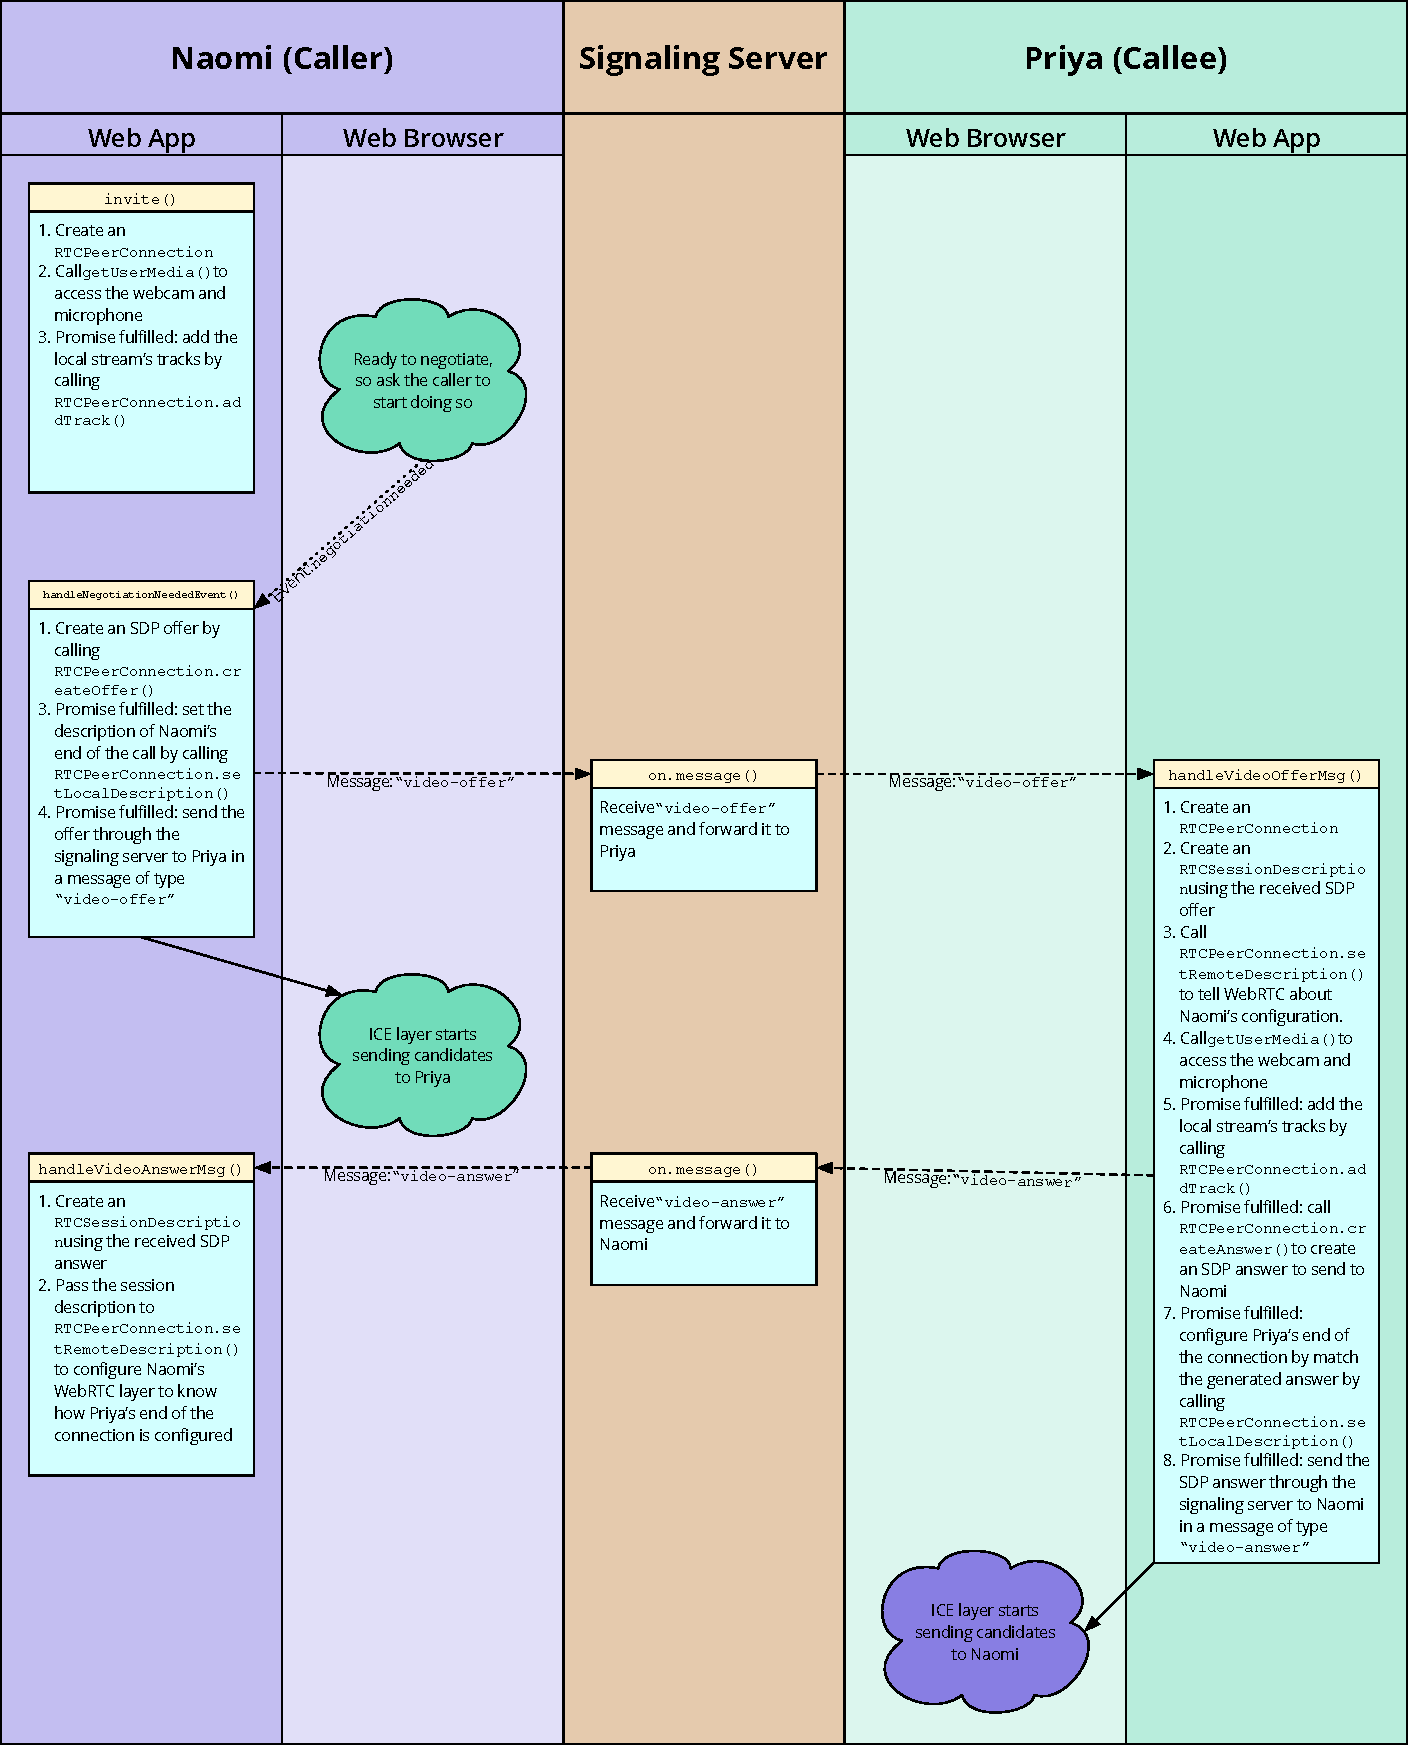
\includegraphics[width=1.4\textwidth,height=1\textheight]{images/SignalingDiagram.pdf}
	\centering
	\caption{Signaling Diagram, \url{https://mdn.mozillademos.org/files/12363/WebRTC - Signaling Diagram.svg}}
	\label{fig:Signaling Diagram}
\end{figure}

There are multiple signaling solutions available, but there are also frameworks available to create custom ones.

For a custom solutions it's handy to use \index{WebSocket}{WebSocket} since it's creating a bidirectional connection between server and client. A handy solution for this use case would be a framework like socket.io~\autocite{socketio} since it's a JavaScript framework it'll work the same on a \index{node}{node} server and client.